\documentclass{homework}

\usepackage{mytoolbox}

\input{particulars}

\renewcommand\thesection{\arabic{section}}
\renewcommand\thesubsection{\arabic{section}.\arabic{subsection}}
\renewcommand\thesubsubsection{\arabic{section}.\arabic{subsection}.\arabic{subsubsection}}

\setlength{\parskip}{0.5em}

\begin{document}

\title{Deep Learning Lab2 \\ Binary Semantic Segmentation}
\author{\chineseName \masterStudentID}
\date{}
\maketitle

\section{Implementation Details}

% Please describe the details of your training, evaluation, and inference code. Explain how the different 
% components  of  your  implementation  work  together  and  highlight  any  important  design  choices. 
% Additionally,  provide  a  detailed  explanation  of  your  models,  specifically  UNet  and  ResNet34_UNet, 
% including architectural modifications, training settings, and optimization strategies. If there are any other 
% relevant  details  that  you  find  important,  you  are  encouraged  to  include  them  in  this  section. 

\subsection{Model Architecture}

\subsubsection{UNet}

For the UNet model, I first implemented the layers:

\begin{itemize}
    \item \lstinline{ConvConv}: Conv2d -> BatchNorm2d -> ReLU -> Conv2d -> BatchNorm2d -> ReLU
    \item \lstinline{Enc}: (Optional) MaxPool2d -> ConvConv
    \item \lstinline{Dec}: ConvTranspose2d -> concat with another tensor -> ConvConv
\end{itemize}

Then, I implemented the UNet model with 1 channel output, which represent the mask probability. The model flow is as follows:

\begin{lstlisting}[language=Python]
    x1 = Enc(3, 64, pooling=False)(x)
    x2 = Enc(64, 128)(x1)
    x3 = Enc(128, 256)(x2)
    x4 = Enc(256, 512)(x3)
    x5 = Enc(512, 1024)(x4)

    x = Dec(1024, 512)(x5, x4)
    x = Dec(512, 256)(x, x3)
    x = Dec(256, 128)(x, x2)
    x = Dec(128, 64)(x, x1)

    x = nn.Conv2d(64, 1, kernel_size=1)(x)
\end{lstlisting}

The numbers in the layer names represent the number of input and output channels.

\subsubsection{ResNet34\_UNet}

The ResNet34\_UNet model uses a ResNet34-style encoder combined with a UNet-style decoder. The encoder is constructed using stacked residual blocks defined via a helper method \lstinline{_make_layer}, which builds layers with optional downsampling and shortcut connections.

\begin{itemize}
    \item \lstinline{_make_layer(in_channels, out_channels, blocks, stride)} constructs a sequence of \lstinline{ResBlock} modules.
    \item Each \lstinline{ResBlock} consists of two \lstinline{Conv2d -> BatchNorm2d -> ReLU} submodules with residual connections.
    \item If the input/output channel count or stride differs, a 1x1 convolution with batch normalization is used as a shortcut.
\end{itemize}

The model flow is as follows:

\begin{lstlisting}[language=Python]
    x = nn.Sequential(
        nn.Conv2d(3, 64, kernel_size=7, stride=2, padding=3),
        nn.BatchNorm2d(64),
        nn.ReLU(),
        nn.MaxPool2d(kernel_size=3, stride=2, padding=1),
    )(x)                                    # (B, 64, 64, 64)
    x1 = _make_layer(64, 64, 3)(x)          # (B, 64, 64, 64)
    x2 = _make_layer(64, 128, 4, 2)(x1)     # (B, 128, 32, 32)
    x3 = _make_layer(128, 256, 6, 2)(x2)    # (B, 256, 16, 16)
    x4 = _make_layer(256, 512, 3, 2)(x3)    # (B, 512, 8, 8)

    x5 = Sequential(
        Conv2d(512, 256, kernel_size=1),
        BatchNorm2d(256),
        ReLU(),
    )(x4)                                   # (B, 256, 8, 8)
    x5 = torch.cat([x5, x4], dim=1)         # (B, 768, 8, 8)

    x = Dec(256 + 512, 32 + 256)(x5, x3)    # (B, 288, 16, 16)
    x = Dec(32 + 288, 32 + 128)(x, x2)      # (B, 160, 32, 32)
    x = Dec(32 + 160, 32 + 64)(x, x1)       # (B, 96, 64, 64)

    x = Sequential(
        ConvTranspose2d(32 + 64, 32, kernel_size=2, stride=2),
        ConvConv(32, 32),
        ConvTranspose2d(32, 32, kernel_size=2, stride=2),
        ConvConv(32, 32),
        Conv2d(32, 1, kernel_size=1),
    )(x)                                    # (B, 1, 256, 256)
\end{lstlisting}

The decoder uses the \lstinline{Dec} blocks with skip connections to fuse encoder features. The final layers upsample the result and apply \lstinline{ConvConv} blocks for refinement.

\subsection{Utilities}

\subsubsection{Dice Score}

The evaluation metric used throughout training and validation is the Dice Score, which measures the overlap between the predicted mask and the ground truth. It is defined as:

\[
\text{Dice} = \frac{2 \cdot |A \cap B| + \epsilon}{|A| + |B| + \epsilon}
\]

Where:
\begin{itemize}
    \item \( A \) is the predicted mask.
    \item \( B \) is the ground truth mask.
    \item \( \epsilon = 10^{-6} \) is a small constant to prevent division by zero.
\end{itemize}

The implementation flattens both tensors, optionally thresholds the predicted probabilities (by default at 0.5), and computes the intersection and union:

\begin{lstlisting}[language=Python]
def dice_score(pred_prob, gt_mask, round=True, threshold=0.5):
    smooth = 1e-6
    pred_prob = pred_prob.flatten()
    if round:
        pred_prob = (pred_prob > threshold).float()
    gt_mask = gt_mask.flatten()
    intersection = (pred_prob * gt_mask).sum()
    union = pred_prob.sum() + gt_mask.sum()
    return (2.0 * intersection + smooth) / (union + smooth)
\end{lstlisting}

This function is used during training, validation, and testing to monitor segmentation performance.

\subsubsection{Overlay Visualization}

To visualize model predictions, I implement the \lstinline{overlay_image()} function, which overlays predicted mask contours (and optionally ground truth) onto the original images. This helps in qualitatively inspecting model performance during training and validation.

\begin{itemize}
    \item Input \lstinline{image}: shape \lstinline{[B, 3, H, W]}, with values in range \lstinline{[0, 255]}.
    \item Input \lstinline{prob}: predicted probability mask, shape \lstinline{[B, 1, H, W]}, values in \lstinline{[0, 1]}.
    \item Optional \lstinline{ground_truth}: ground truth binary mask.
\end{itemize}

The function does the following:

\begin{enumerate}
    \item Transposes the image to \lstinline{[B, H, W, 3]} for OpenCV compatibility.
    \item Binarizes the probability mask at 0.5 threshold and extracts contours.
    \item Draws prediction contours in yellow.
    \item If provided, draws ground truth contours in green.
\end{enumerate}

\subsection{Training}

\subsubsection{Argument Parsing}
I use \lstinline{argparse} to configure the training process. The function \lstinline{get_args()} defines options such as:

\begin{itemize}
    \item \lstinline{--debug}: Enables debugging mode.
    \item \lstinline{--data_path}: Path to dataset (default: \lstinline{dataset/oxford-iiit-pet}).
    \item \lstinline{--experiment_name}: Custom name for the experiment (default: timestamp-based).
    \item \lstinline{--model}: Selects the model (\lstinline{unet} or \lstinline{resnet34_unet}).
    \item \lstinline{--epochs}, \lstinline{--batch_size}, \lstinline{--learning-rate}: Training parameters.
\end{itemize}

These values are post-processed to generate a unique \lstinline{experiment_name} for logging and checkpoint management.

\subsubsection{Comet.ml Logging}
I integrate Comet.ml for experiment tracking. If \lstinline{COMET_API_KEY} is set and \lstinline{--debug} is not enabled:

\begin{itemize}
    \item An experiment is created with project/workspace settings from environment variables.
    \item Arguments are logged with \lstinline{log_parameters(vars(args))}.
    \item Metrics (train/val/test dice and loss) are logged each epoch.
    \item Visual outputs (mask predictions) are logged as images.
\end{itemize}

The experiment can be viewed at \\
\url{https://www.comet.com/jteng2127/dlp-lab2?shareable=B9TjiraiLlmSx9KMEory3ThVa}.

\subsubsection{Debug Mode}
When \lstinline{--debug} is used:

\begin{itemize}
    \item Logging is disabled.
    \item Model saving is skipped.
    \item A remote debugger (debugpy) is attached to port 5678 to support step-wise inspection.
\end{itemize}

\subsubsection{Training Procedure}
The \lstinline{train(args)} function performs the following:

\begin{enumerate}
    \item Loads datasets with Albumentations-based augmentation for training.
    \item Initializes the selected model and optimizer (\lstinline{Adam}).
    \item Defines the loss as \lstinline{BCEWithLogitsLoss} and uses Dice Score for evaluation.
    \item For each epoch:
    \begin{itemize}
        \item Performs forward and backward passes.
        \item Logs visual outputs for the first batch to Comet.
        \item Evaluates on validation set and saves best model based on validation Dice score.
    \end{itemize}
    \item After training, evaluates the model on the test set and logs the final Dice score.
\end{enumerate}

\subsubsection{Environment Configuration}
Environment variables like \lstinline{COMET_API_KEY} and related settings are configured in \lstinline{.env} files. The \lstinline{python-dotenv} package is used to load these settings:

\begin{lstlisting}[language=Python]
dotenv.load_dotenv()
\end{lstlisting}

\subsection{Evaluation}

After training, I use a evaluation script to measure the Dice Score on the train, validation, and test sets. The evaluation pipeline performs the following:

\begin{enumerate}
    \item Loads the model architecture and weights:
    \begin{itemize}
        \item If \lstinline{--epochs} is provided, loads \lstinline{model_<epochs>.pth}.
        \item Otherwise, loads the best model checkpoint \lstinline{model_best.pth}.
    \end{itemize}
    \item Initializes datasets and wraps them with \lstinline{DataLoader} for inference.
    \item Uses the \lstinline{evaluate()} function:
    \begin{itemize}
        \item Sets the model to evaluation mode.
        \item Iterates through the loader, runs inference, and computes average Dice Score.
    \end{itemize}
    \item Prints Dice scores for each data split.
\end{enumerate}

The following code snippet summarizes the evaluation procedure:

\begin{lstlisting}[language=Python]
model.load(model_path)

train_dice = evaluate(model, train_loader, device)
print(f'Train Dice: {train_dice:.4f}')

valid_dice = evaluate(model, valid_loader, device)
print(f'Valid Dice: {valid_dice:.4f}')

test_dice = evaluate(model, test_loader, device)
print(f'Test Dice: {test_dice:.4f}')
\end{lstlisting}

\subsection{Inference}

\subsubsection{Inference Script}

The inference script generates predicted masks and visualizations from a trained model. It supports both \lstinline{UNet} and \lstinline{ResNet34_UNet} models and loads weights from either \lstinline{model_best.pth} or a specific epoch.

Arguments are parsed via \lstinline{argparse}, including:
\begin{itemize}
    \item \lstinline{--experiment_name}: Used to locate model checkpoints.
    \item \lstinline{--model_dir}, \lstinline{--output_dir}: For checkpoint and prediction output directories.
    \item \lstinline{--model}, \lstinline{--epochs}, \lstinline{--batch_size}: For inference control.
\end{itemize}

\subsubsection{Overlay and Saving Predictions}

The \lstinline{inference()} function performs the following:

\begin{enumerate}
    \item Runs the model in evaluation mode.
    \item Applies \lstinline{torch.sigmoid()} to convert logits to probabilities.
    \item Calls \lstinline{overlay_image()} to visualize predicted and ground truth contours.
    \item Saves overlaid images to disk using \lstinline{PIL.Image}.
\end{enumerate}

Outputs are saved to:
\begin{itemize}
    \item \lstinline{output/<full_experiment_name>/train}
    \item \lstinline{output/<full_experiment_name>/valid}
    \item \lstinline{output/<full_experiment_name>/test}
\end{itemize}

\section{Data Preprocessing (Data Augmentation)}

To improve generalization, I apply data augmentation using \lstinline{Albumentations}. The training images and masks are transformed with:

\begin{lstlisting}[language=Python]
train_transform = A.Compose([
    A.HorizontalFlip(p=0.5),
    A.ColorJitter(p=0.2),
])
\end{lstlisting}

\begin{itemize}
    \item \lstinline{HorizontalFlip(p=0.5)}: Randomly flips the image and mask horizontally with 50\% probability.
    \item \lstinline{ColorJitter(p=0.2)}: Randomly changes image brightness, contrast, and saturation with 20\% probability (applied to image only, not mask).
\end{itemize}

These augmentations help the model become more robust to positional and illumination changes. No augmentations are applied to validation and test sets to ensure consistent evaluation.

\section{Analyze the experiment results}

\subsection{Best Model}

For the best model of Unet and ResNet34\_Unet, I obtain the following Dice scores:

\begin{table}[H]
    \centering
    \begin{tabular}{|c|c|c|c|}
        \hline
        Model & Train Dice & Valid Dice & Test Dice \\
        \hline
        UNet (w/ Aug, w/ BN) & 0.9703 & 0.9335 & 0.9307 \\
        ResNet34\_UNet (w/ Aug, w/ BN) & 0.9726 & 0.9264 & 0.9272 \\
        \hline
    \end{tabular}
\end{table}

Where \textit{Aug} denotes data augmentation and \textit{BN} denotes batch normalization.

The settings of the best models are as follows:

\begin{table}[H]
    \centering
    \begin{tabular}{|c|c|c|c|}
        \hline
        Model & Best Epoch & Batch Size & Learning Rate \\
        \hline
        UNet (w/ Aug, w/ BN) & 52 & 8 & 0.0001 \\
        ResNet34\_UNet (w/ Aug, w/ BN) & 60 & 8 & 0.0001 \\
        \hline
    \end{tabular}
\end{table}

The training curve of the best models is shown in the following figure:

\begin{figure}[H]
        \centering
        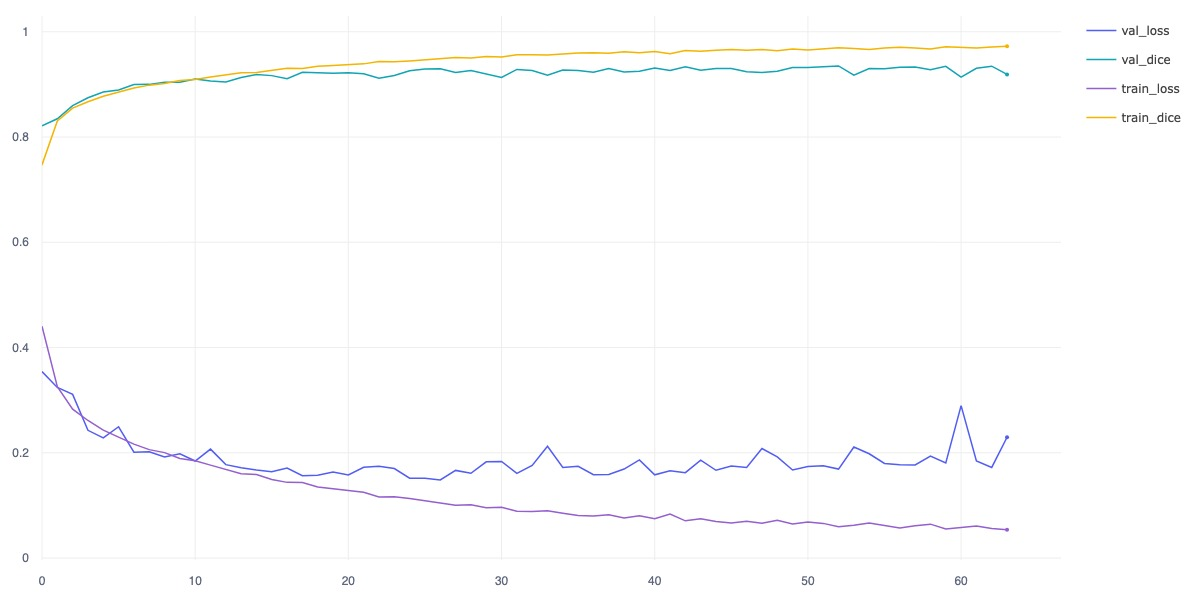
\includegraphics[width=0.9\textwidth]{unet_train_curve.jpg}
        \caption{UNet training curve}
\end{figure}

\begin{figure}[H]
    \centering
    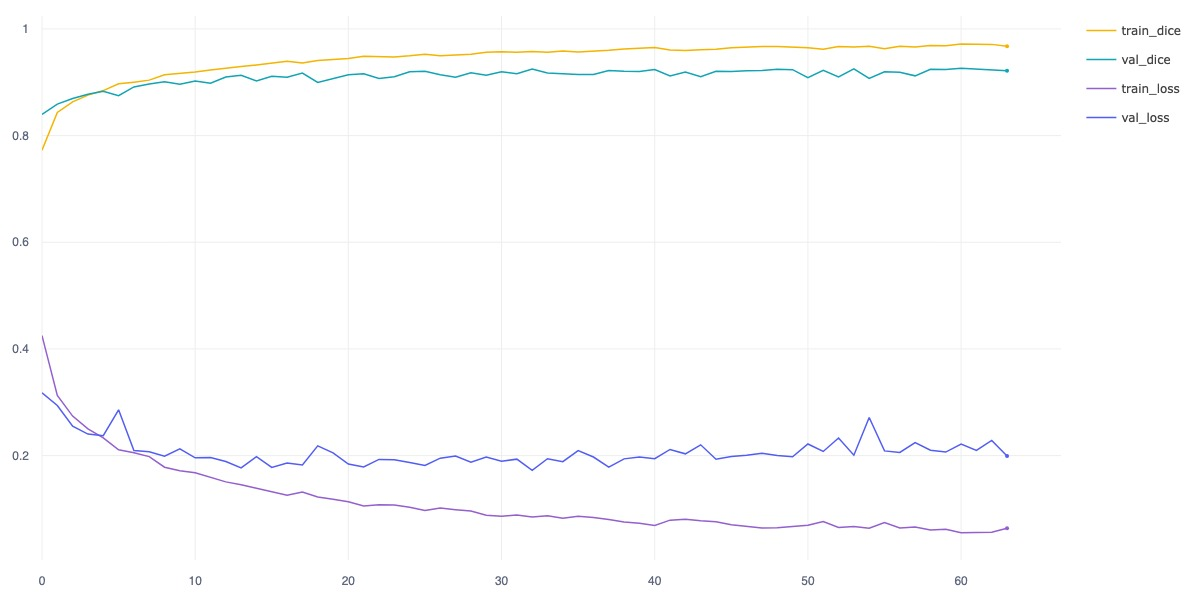
\includegraphics[width=0.9\textwidth]{resnet34_unet_train_curve.jpg}
    \caption{ResNet34\_UNet training curve}
\end{figure}

\subsection{Abalation Study}
 
I compare the result of the models with and without data augmentation and batch normalization. The results are as follows:

\begin{table}[H]
    \centering
    \begin{tabular}{|c|c|c|c|}
        \hline
        Model & Train Dice & Valid Dice & Test Dice \\
        \hline
        UNet (w/ Aug, w/ BN) & 0.9703 & 0.9335 & 0.9307 \\
        UNet (w/o Aug, w/ BN) & 0.9703 & 0.9225 & 0.9214 \\
        UNet (w/o Aug, w/o BN) & 0.8395 & 0.8339 & 0.8342 \\
        \hline
        ResNet34\_UNet (w/ Aug, w/ BN) & 0.9726 & 0.9264 & 0.9272 \\
        ResNet34\_UNet (w/o Aug, w/ BN) & 0.9734 & 0.9123 & 0.9153 \\
        \hline
    \end{tabular}
\end{table}

From the table, I observe several key findings:

\begin{itemize}
    \item \textbf{Data Augmentation}: Improves validation and test performance in both UNet and ResNet34\_UNet. For example, in UNet, augmentation improves test Dice from 0.9214 to 0.9307.
    \item \textbf{Batch Normalization}: Has a significant impact. Removing BN from UNet causes a large drop in all scores (e.g., test Dice from 0.9214 to 0.8342), indicating BN is essential for stable training and convergence.
\end{itemize}

These results confirm that both augmentation and batch normalization are beneficial for generalization. Batch Normalization is essential because it stabilizes training by normalizing activations, which improves gradient flow, allows faster convergence, and acts as a form of regularization.

\subsection{Visualizations}

The following figures show visualizations of the model predictions on the test set:

\begin{figure}[H]
    \centering
    \begin{subfigure}{0.20\textwidth}
        \centering
        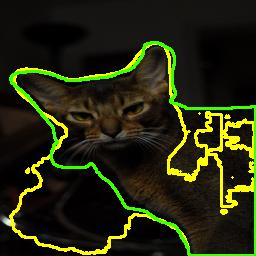
\includegraphics[width=0.9\textwidth]{Unet_Abyssinian_4.jpg}
        \caption{UNet test 1}
    \end{subfigure}
    \begin{subfigure}{0.20\textwidth}
        \centering
        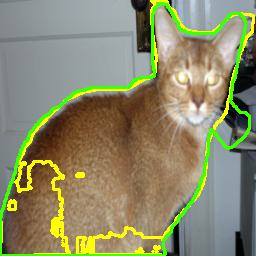
\includegraphics[width=0.9\textwidth]{Unet_Abyssinian_27.jpg}
        \caption{UNet test 2}
    \end{subfigure}
    \begin{subfigure}{0.20\textwidth}
        \centering
        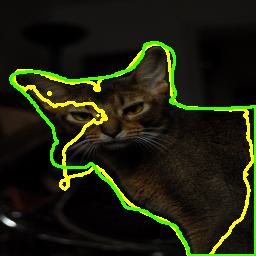
\includegraphics[width=0.9\textwidth]{ResNet34_Unet_Abyssinian_4.jpg}
        \caption{ResUNet test 1}
    \end{subfigure}
    \begin{subfigure}{0.20\textwidth}
        \centering
        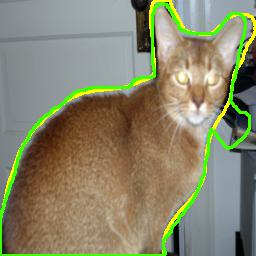
\includegraphics[width=0.9\textwidth]{ResNet34_Unet_Abyssinian_27.jpg}
        \caption{ResUNet test 2}
    \end{subfigure}
    \caption{Test set predictions}
    \label{fig:qualitative}
\end{figure}

The yellow contours represent the predicted masks, while the green contours represent the ground truth. The visualizations show that both models can mostly segment the pets correctly, with some minor errors.

\section{Execution steps}

For training, follow these steps:

\begin{enumerate}
    \item Prepare the environment via \lstinline{pip install -r requirements.txt}.
    \item Download the dataset from \url{https://www.robots.ox.ac.uk/~vgg/data/pets/}, extract it to \lstinline{dataset/oxford-iiit-pet}.
    \item (Optional) If you want to record on Comet.ml, copy the \lstinline{.env.example} file to \lstinline{.env} and set your Comet information.
    \item Run \lstinline{python src/train.py -e 32 -b 8 -l 1e-4 -n <experiment_prefix> -m <unet|resnet34_unet>} to train the UNet model, with 32 epochs, batch size 8, learning rate 0.0001, and experiment name prefix \lstinline{<experiment_prefix>}. The model will be saved to \lstinline{saved_models/<full_experiment_name>/model_best.pth}.
\end{enumerate}

For evaluation and inference, use the following commands:

\begin{enumerate}
    \item Run \lstinline{python src/evaluate.py -n <full_experiment_name> -m <unet|resnet34_unet>} to evaluate the model.
    \item Run \lstinline{python src/inference.py -n <full_experiment_name> -m <unet|resnet34_unet>} to generate predictions. The results will be saved to \lstinline{output/<full_experiment_name>/<train|valid|test>}.
\end{enumerate}

\section{Discussion}

\subsection{Model Comparison}

We can observe that while both models perform well, there are subtle differences in their behavior:

\begin{itemize}
    \item \textbf{UNet} achieves higher validation and test Dice scores, suggesting better generalization on this dataset. It converges slightly faster (best at epoch 52).
    \item \textbf{ResNet34\_UNet} has the highest train Dice, indicating strong fitting capacity, but its generalization is slightly weaker, possibly due to overfitting or increased model complexity.
\end{itemize}

This suggests that while deeper backbones like ResNet34 provide stronger representational power, plain UNet remains more effective when data is limited or relatively simple, benefiting from fewer parameters and a more straightforward architecture.

\subsection{Data Augmentation Trade-offs}

While data augmentation improves model generalization, it also introduces training instability. Specifically, I observe the following effects during training:

\begin{itemize}
    \item \textbf{Train Dice Score}: Slightly lower than models trained without augmentation, due to increased input variance.
    \item \textbf{Validation and Test Dice Scores}: Slightly improved, indicating better generalization and robustness to unseen variations.
    \item \textbf{Convergence Speed}: Slower convergence, requiring approximately twice as many epochs to reach optimal performance compared to training without augmentation.
\end{itemize}

This trade-off is expected, as augmented data introduces more variability, making the learning task harder but also reducing overfitting.

\subsection{Dataset Issues}

The Oxford-IIIT Pet dataset is relatively small and simple, containing only pet images with binary segmentation masks. 

However, the dataset also contains pixels labeled as \textbf{"Not Classified"} in the original annotation masks. In our implementation, we treat all non-background pixels—including these "Not Classified" regions—as valid foreground annotations.

For example, in the ground truth of test image 2 shown in Figure~\ref{fig:qualitative}, the \textbf{"Not Classified"} pixels appear in the cat's whisker region. Including them as foreground introduces noise, as they do not consistently represent object boundaries and can mislead the model during training.

\end{document}